\section{Marco teórico}
\vspace{5 px}
Un sistema aéreo no tripulado está compuesto por (ver figura \ref{fig:UAS}): una o varias aeronaves, denominadas Vehículos Aéreos No Tripulados (UAV), sus cargas útiles, las estaciones de control en tierra (y, a menudo, otras estaciones remotas), sistemas de lanzamiento y recuperación de aeronaves, sistemas de soporte, comunicación, transporte y el componente humano requerido para su operación\cite{UAS-FAC}.  \\



La arquitectura de un Sistema Aéreo No Tripulado (UAS) integra múltiples componentes esenciales para su funcionamiento eficiente y seguro. Los UAVs son las plataformas aéreas del sistema, equipadas con sistemas de propulsión, navegación, y control, así como diversas cargas para misiones específicas, como cámaras, sensores térmicos o equipos de recolección de datos ambientales. La estación de control en tierra (GCS) es el núcleo operativo del UAS, donde los operadores supervisan y dirigen el vuelo del UAV, analizan la información recibida y toman decisiones críticas durante la misión. Los sistemas de comunicación, que pueden incluir enlaces satelitales y de radiofrecuencia, aseguran una transmisión de datos continua y fiable entre el UAV y la estación de control, permitiendo un control preciso y seguro del vehículo en diversas condiciones operativas \cite{UAS-FAC}. \\

\begin{figure}[H]
    \centering
    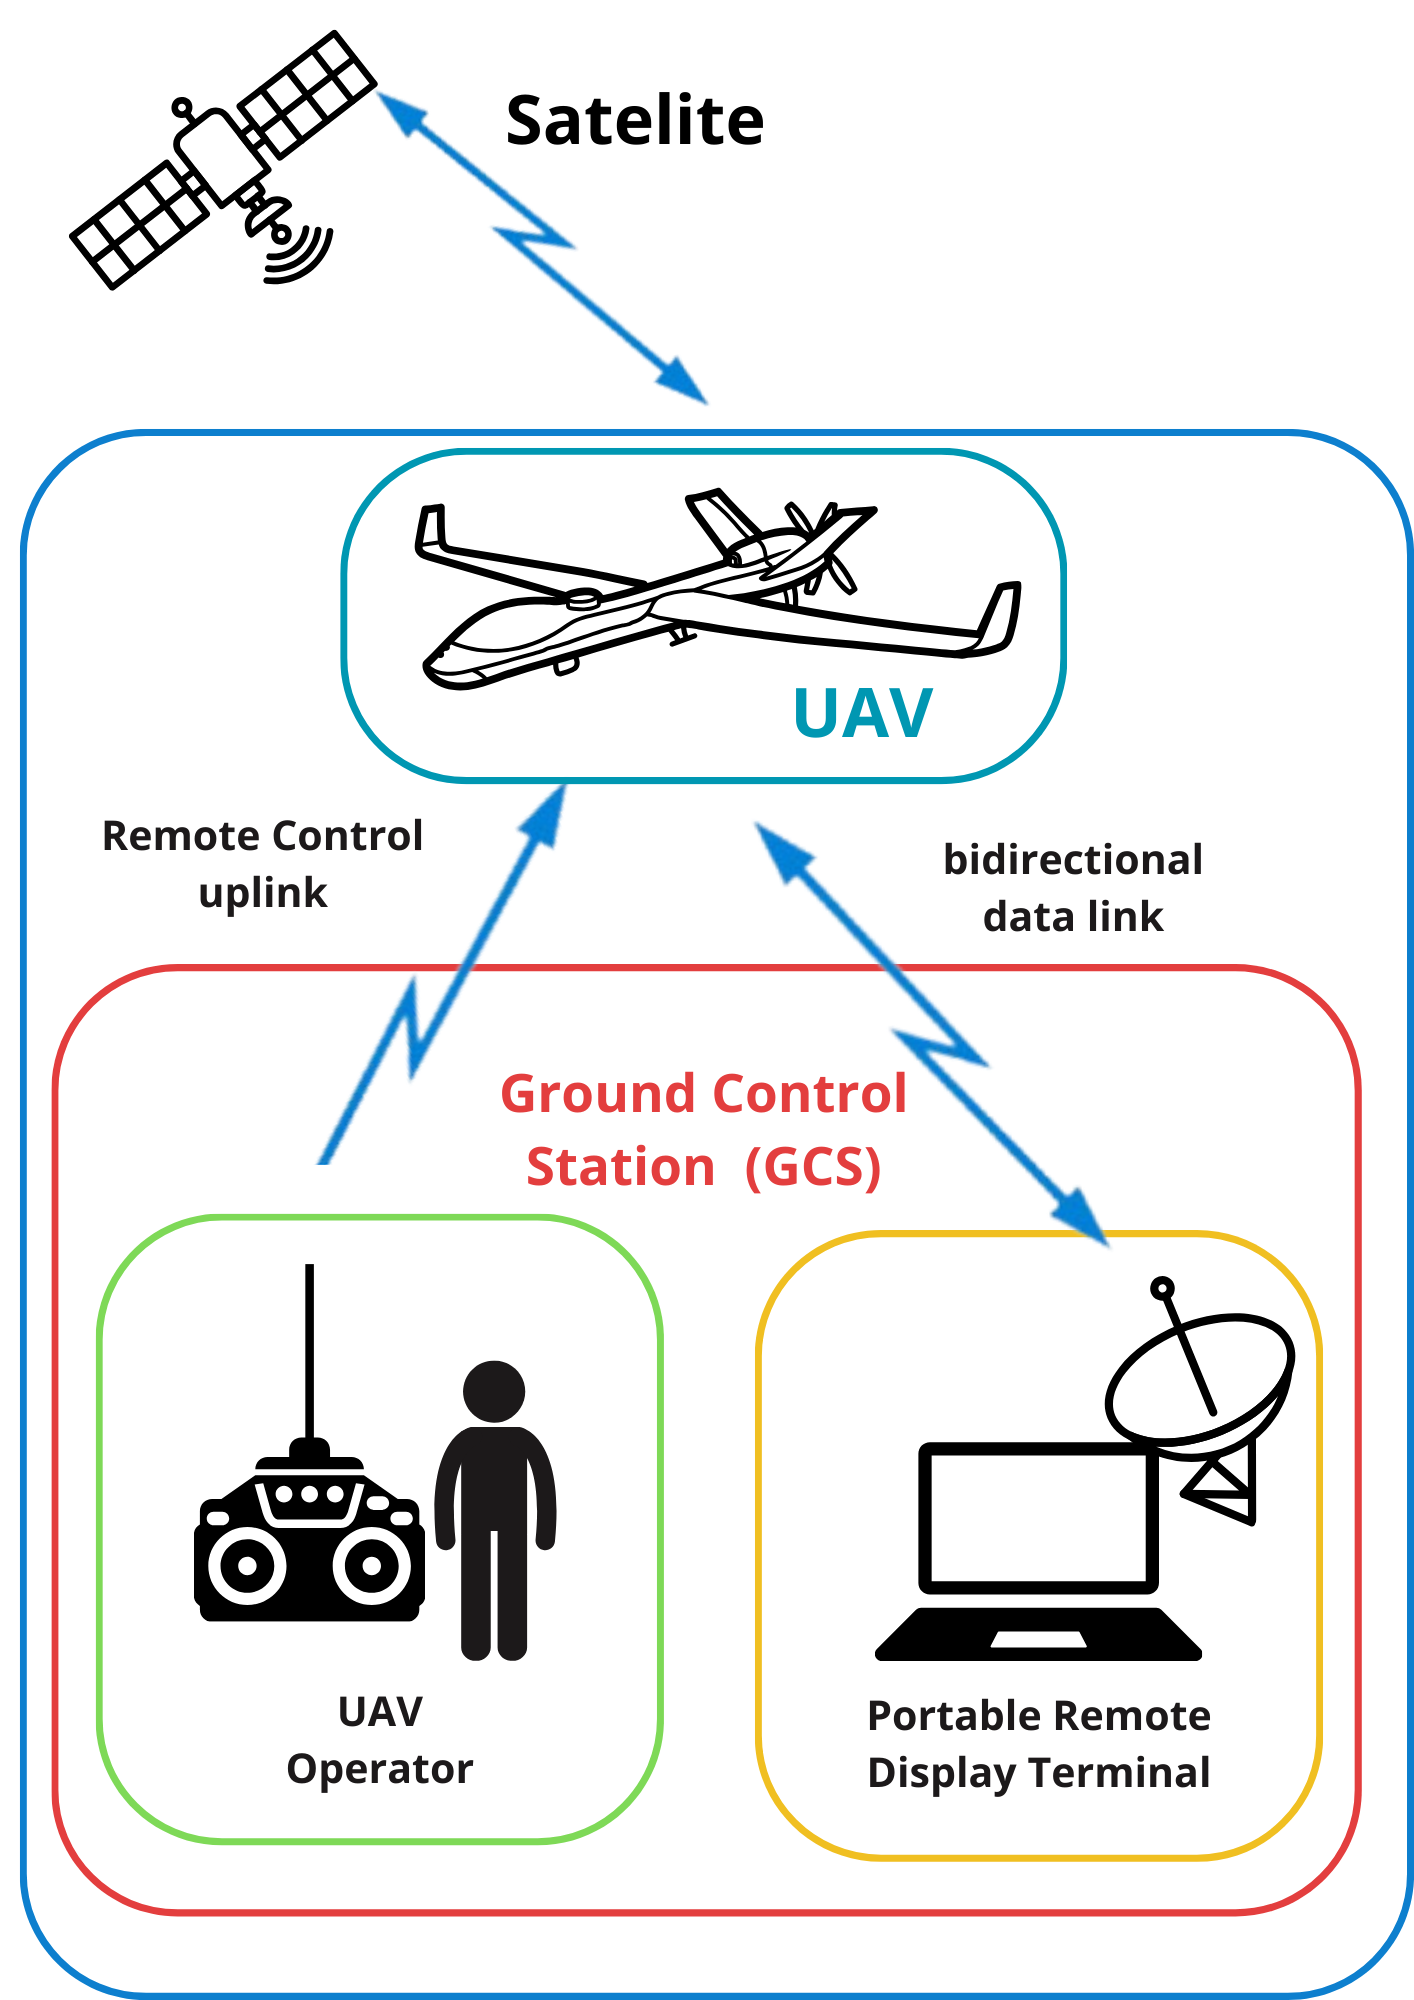
\includegraphics[width=10cm, height=12cm]{Imagenes/Marco Teorico/UAS.png}
    \caption{ Sistema aéreo no tripulado (UAS)}
    \label{fig:UAS}
\end{figure}


El subsistema de comunicación es crucial en esta arquitectura, ya que asegura la transmisión bidireccional de datos entre el UAV y la GCS. Este sistema puede incluir enlaces de radiofrecuencia, satelitales y otros métodos de comunicación redundantes para garantizar la conectividad continua y la seguridad operativa. Una condición importante a tener en cuenta es que los UAS se diseñan para ser operados sin tripulación a bordo de la aeronave. Esto impone la demanda de un control o una unidad de toma de decisiones que debe asumir esta responsabilidad. La combinación de estos elementos permite a los UAS realizar misiones complejas y prolongadas, proporcionando una plataforma flexible y robusta para una amplia gama de aplicaciones \cite{UAS-FAC}.



\subsection{UAV}
Un Vehículo Aéreo No Tripulado (UAV), comúnmente conocido como drone, es una aeronave sin tripulación humana a bordo que requiere un sistema de control eficiente para llevar a cabo una variedad de tareas. Estas tareas pueden incluir misiones de vigilancia, mapeo, entrega de carga, inspección, entre otras \cite{UAV1}.



\vspace{5 px}
\subsubsection{ UAV de ala fija}
Los Vehículos Aéreos No Tripulados (UAV) de ala fija, también conocidos como drones de ala fija, se caracterizan por sus alas sin movimiento rotacional y su incapacidad para volar verticalmente \cite{alafija}. A diferencia de los drones multirotor, estos UAVs ofrecen ventajas significativas, como mayor seguridad al no tener hélices giratorias constantes, una mayor eficiencia en el vuelo gracias a su capacidad para planear con el aire, mayor autonomía de vuelo debido a un menor consumo de batería, y la capacidad de cubrir áreas extensas \cite{UAV2}. Además, son resistentes a condiciones climáticas adversas y tienen un costo más económico en comparación con otros tipos de drones. Sin embargo, requieren un espacio amplio para el despegue y el aterrizaje, lo que los hace ideales para aplicaciones que involucran exploración extensa y operaciones en terrenos variados \cite{alafija}.

\begin{figure}[H]
    \centering
    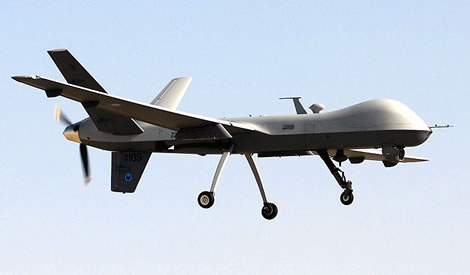
\includegraphics[width=8cm, height=5cm]{Imagenes/Marco Teorico/raf_reaper_fly.jpg}
    \caption{Dron de ala fija MQ-9 Reaper Hunter \cite{reaper}}
    \label{fig:enter-label}
\end{figure}


\subsection{Ground Control Station (GCS):}

La Ground Control Station (GCS) es una parte integral de los Sistemas de Aeronaves No Tripuladas (UAS) que desempeña un papel crucial en la operación y control del UAV. Según la referencia de la Fuerza Aérea Colombiana \cite{UAS-FAC}, la GCS se compone de dos componentes principales: \\

\subsubsection{Interfaz de la GCS:}

Terminal de Visualización Remota Portátil: Esta interfaz proporciona a los operadores una plataforma para monitorizar y controlar el UAV. Incluye pantallas y dispositivos de entrada que permiten la visualización en tiempo real de los datos de vuelo y la telemetría del UAV, así como la capacidad de enviar comandos al UAV. La interfaz es esencial para la gestión de misiones y la toma de decisiones durante el vuelo. \\
:

\subsubsection{Operador del UAV:} El operador es responsable de la supervisión directa y el control del UAV a través de la GCS. Utiliza dispositivos de control remoto y la interfaz de la GCS para dirigir el vuelo, realizar ajustes en tiempo real y responder a cualquier eventualidad que pueda surgir durante la operación del UAV. El operador aéreo debe estar entrenado y ser competente en el manejo de los sistemas y procedimientos del UAS.\\

\subsection{Controlador de Vuelo}
\vspace{5 px}

Un controlador de vuelo consiste esencialmente en un circuito electrónico con distintos componentes electrónicos tales como micro-chips, condensadores, capacitores, resonadores, inductores, entre otros. Este dispositivo se comporta en esencia como el cerebro de un drone, puesto que tiene un procesador que computa todos los datos referentes a la aeronave y ejecuta acciones de control en el vuelo. Además, posee un software que supervisa las acciones del drone. Las funciones del controlador puedene ser dividas en tres categorías principales: percepción, control y comunicación \cite{6}.\\

En el ámbito de la percepción, el controlador de vuelo se enlaza con una serie de sensores que proveen información vital, como la altura, orientación y velocidad del dron. Estos sensores incluyen unidades de medición inercial (IMU) para calcular la velocidad angular y la aceleración, barómetros para la altitud y sensores de distancia para detectar obstáculos. El controlador procesa y combina esta información sensorial para generar acciones de control eficaces y precisas \cite{6}. \\

Por otro lado, en el ámbito de control el controlador de vuelo efectúa las acciones de movimiento del dispositivo, regulando el movimiento de los distintos actuadores del UAV, tales como motores y servomotores para regular las dinámicas de vuelo de la aeronave. Es importante tener en cuenta que en la creación de un controlador de vuelo para UAV de ala fija, se debe diseñar un sistema capaz de gestionar de manera precisa y coordinada los alerones, timón y cola de la aeronave. Esto implica la necesidad de un control preciso de las superficies de control del UAV, como los alerones para el balanceo, el timón para el giro y la cola para el control de cabeceo, para garantizar una navegación estable y maniobras precisas en vuelo. \\

Por su parte, en el ámbito de comunicaciones, el controlador de vuelo es capaz de comunicarse en tierra con la estación en base. De tal forma que se pueda efectuar una comunicación bidireccional entre el operador de vuelo y el UAV. Además, requiere la integración de un sistema de posicionamiento por satélite (GPS) para conocer la posición en tiempo real del UAV.\\

\vspace{5 px}

\begin{figure}[H]
    \centering
    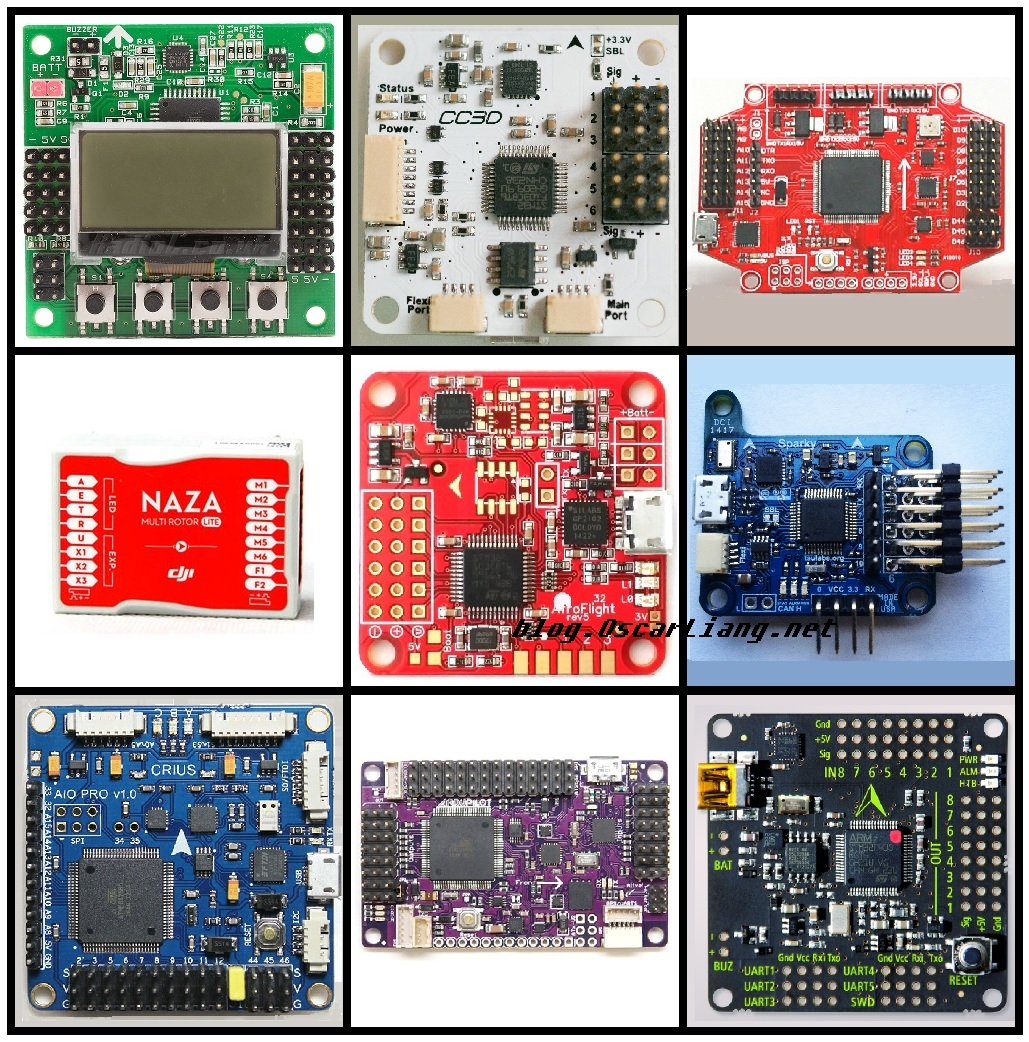
\includegraphics[width=8cm, height=5cm]{Imagenes/Marco Teorico/flight controller.jpg}
    \caption{Controladores de Vuelo \cite{controladores}}
    \label{fig:enter-label}
\end{figure}

%%\subsection{Algoritmo de Seguimiento de Trayectorias}



%En la navegación autónoma, los UAV de ala fija se orientan hacia un punto de referencia visible, conocido como waypoint, para dirigirse a su destino. El algoritmo "line-of-sight" (LOS) es clave en este proceso, particularmente en situaciones de "control underactuated", donde los UAV tienen más grados de libertad que actuadores disponibles para controlar esos movimientos \cite{7}.

%El algoritmo LOS opera calculando un vector de dirección desde la posición actual del UAV hasta el waypoint. Este vector guía al UAV, permitiéndole ajustar continuamente su trayectoria mediante cambios en las superficies de control (alerón, timón, elevador) y la fuerza de empuje. A medida que el UAV se mueve, el algoritmo recalcula el vector en función de la nueva posición y realiza los ajustes necesarios.

%Por ejemplo, si un UAV se desvía de su ruta debido a una ráfaga de viento, el sistema LOS identificará la diferencia entre la posición actual y el waypoint deseado. Luego, calculará un nuevo vector de dirección y emitirá comandos para que el UAV ajuste su vuelo, realineándose con el waypoint.

%%Esta técnica es eficaz para mantener una trayectoria precisa y simplifica el proceso de control, haciendo que sea más fácil para los UAVs navegar hacia y entre waypoints de manera autónoma. La imagen \ref{fig:waypoints} ilustra este concepto con vectores y ángulos que demuestran cómo el UAV se ajusta en dos puntos de tiempo diferentes para alcanzar el waypoint final.



%\begin{figure}[H]
    %\centering
    %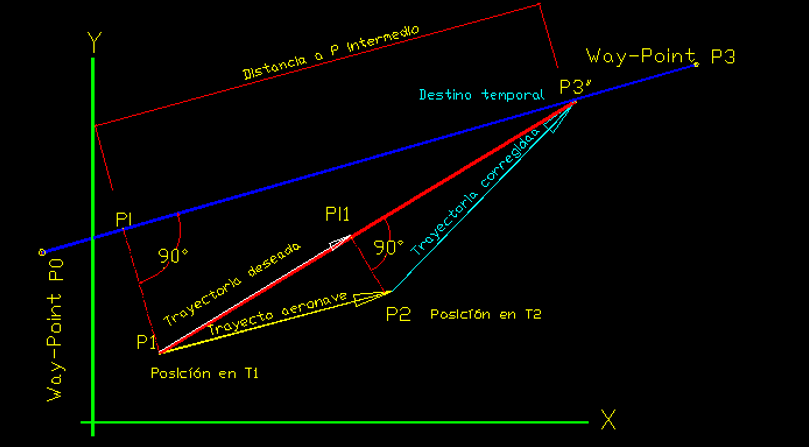
\includegraphics[width=10cm, height=6cm]{Imagenes/Marco Teorico/waitpoints.png}
    %\caption{Esquema de Waypoints para Navegación Autónoma por Jorge Humberto %Rocca}
    %\label{fig:waypoints}
%\end{figure}

\subsection{Ejes inerciales del avión}

Los ejes de simetría de un avión se conocen como: \textit{yaw, pitch y roll}. Estos términos se refieren a las tres dimensiones en las que una aeronave en vuelo puede rotar. Estos ejes, que se mueven y rotan con el vehículo, son fundamentales para el control y la maniobrabilidad de una aeronave. \cite{UAV2}
\vspace{5 px}

\subsubsection{Yaw o eje vertical:} Este eje va de arriba abajo, perpendicular a los otros dos ejes y paralelo al fuselaje. El movimiento alrededor de este eje se denomina \textit{yaw}, y un movimiento positivo en esta dirección mueve la nariz de la aeronave hacia la derecha, siendo el timón la principal superficie de control.\cite{UAV2}
\vspace{5 px}
\subsubsection{Pitch o eje transversal:} Extendiéndose de izquierda a derecha desde la perspectiva del piloto y paralelo a las alas, este eje controla el movimiento de \textbf{pitch}. Un movimiento positivo eleva la nariz de la aeronave y baja la cola, siendo controlado principalmente por las elevaciones.\cite{UAV2}\\

\subsubsection{Roll o eje longitudinal:} Este eje recorre la aeronave de cola a nariz, en la dirección normal de vuelo. El movimiento alrededor de este eje, conocido como \textit{roll}, implica levantar un ala mientras se baja la otra. Los alerones son los principales controladores de este movimiento, aunque el timón también puede influir secundariamente.\cite{UAV2}\\

Los movimientos alrededor de estos ejes son producidos por torques o momentos, que en las aeronaves se generan intencionalmente mediante el movimiento de superficies de control. Las elevaciones en la cola horizontal controlan el \textit{pitch}, el timón en la cola vertical controla el \textit{yaw}, y los alerones en las alas, que se mueven en direcciones opuestas, controlan el \textit{roll}. En el caso de las naves espaciales, estos movimientos suelen ser producidos por un sistema de control de reacción que utiliza pequeños propulsores para aplicar empuje asimétrico.\cite{UAV2}

\begin{figure}[H]
    \centering
    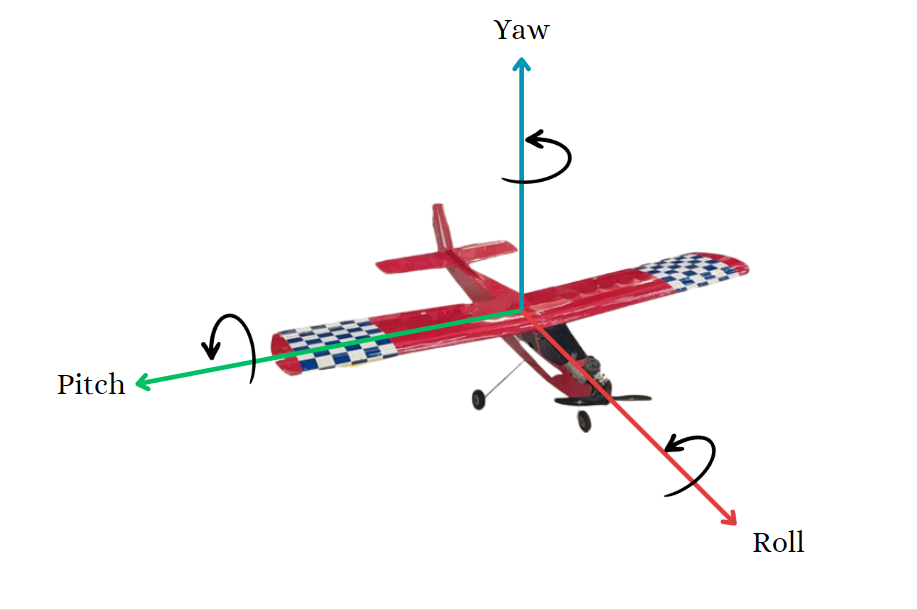
\includegraphics[width=10cm, height=6cm]{Imagenes/Marco Teorico/YAW_PITCH_ROLL_UAV.png}
    \caption{Movimientos Inerciales de un UAV: Yaw, Pitch, Roll}
    \label{fig:waypoints}
\end{figure}



\subsection{Main control unit (MCU)}
Una MCU, o unidad de control principal, es una plataforma integrada que alberga un procesador, memoria y múltiples pines para la interacción con el entorno. En UAVs, la MCU es crucial para la lectura de señales de los sensores, como GPS y giroscopios, y para el envío de comandos a los actuadores del vehículo, permitiendo así el vuelo autónomo y la navegación precisa. \cite{MCU}


\subsection{Unidad de Medida Inercial (IMU)}
Una Unidad de Medida Inercial (IMU) es un dispositivo electrónico que mide y reporta la velocidad angular y la aceleración de un objeto para determinar su orientación y velocidad de movimiento. Principalmente, la IMU se utiliza en la navegación de aeronaves, UAVs, misiles y satélites, operando de manera independiente y libre de interferencias de sistemas externos. Está compuesta por acelerómetros, giróscopos y magnetómetros, los cuales, mediante el uso de algoritmos de fusión de sensores, ayudan a proporcionar datos garantizados sobre la actitud, posición y velocidad, lo que resulta en una alta fiabilidad del sistema contra posibles fallos de los sensores. \cite{IMU}

\subsection{Superficies de control}

Las superficies de control son componentes aerodinámicos móviles esenciales en la aviación, cuya manipulación permite al piloto modificar la aerodinámica del avión para lograr el desplazamiento deseado sobre sus ejes y seguir la trayectoria de vuelo establecida. Existen tres tipos principales de superficies de control: alerones, elevadores y el timón de dirección. Cada una de estas superficies es responsable del control del movimiento en torno a un eje específico del avión. \\
\begin{figure}[H]
    \centering
    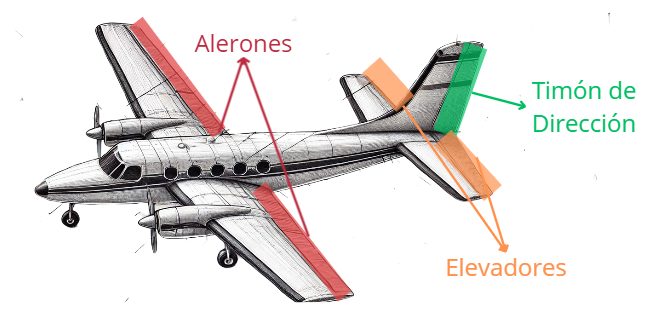
\includegraphics[width=10cm, height=6cm]{Imagenes/Marco Teorico/s_control.png}
    \caption{Superficies de control en una aeronave}
    \label{fig:waypoints}
\end{figure}


\subsection{Sistema de Posicionamiento Global (GPS) }

El GPS (Sistema de Posicionamiento Global) permite la ubicación geográfica de cualquier objeto en el mundo mediante la triangulación de señales en una red de satélites. Este sistema es crucial en la navegación precisa y el control de vuelo de los UAVs (Vehículos Aéreos No Tripulados), ya que les permite conocer su posición exacta en tiempo real. \cite{GPS}

\subsection{Indicadores de vuelo}

Los indicadores de vuelo proporcionan información fundamental sobre las condiciones y la orientación del UAV, permitiendo a los operadores realizar ajustes necesarios para asegurar una operación de vuelo en condiciones seguras. En este proyecto, hemos implementado los siguientes indicadores de vuelo:\\

\begin{itemize}
  \item \textbf{Anemómetro:} Este dispositivo mide la velocidad del aire en relación con el UAV. Es crucial para determinar la velocidad relativa del UAV y ajustar la velocidad de vuelo para mantener un control adecuado y eficiente.\\

  \item \textbf{Horizonte Artificial:} Este indicador muestra la orientación del UAV en relación con el horizonte terrestre. Es fundamental para mantener el equilibrio y la estabilidad durante el vuelo, proporcionando información sobre el ángulo de inclinación y el cabeceo del UAV.\\

  \item \textbf{Altímetro:} El altímetro mide la altitud del UAV sobre el nivel del mar. Esta información es vital para mantener el UAV a una altura segura y para cumplir con las regulaciones de espacio aéreo.\\

  \item \textbf{Indicador de Dirección:} Este dispositivo muestra la dirección del vuelo en relación con el norte geográfico. Es esencial para la navegación y para seguir una ruta de vuelo planificada.\\

  \item \textbf{Indicador de Altitud:} Similar al altímetro, este indicador proporciona información sobre la altitud, pero está calibrado para mostrar variaciones más precisas y rápidas en la altitud del UAV, lo cual es útil para maniobras precisas y ajustes rápidos.\\
\end{itemize}

\subsection{Normativa seguida en el desarrollo del proyecto}

En el desarrollo del proyecto se siguieron los conceptos y esquemas propuestos en la Circular 328-AN/190 de la OACI \cite{circular_aerea}. Conforme a la normativa, se implementaron sistemas de mando y control (C2) fiables, asegurando la capacidad del piloto remoto para operar el UAV de manera segura y eficiente en todo momento.\\

Se tomaron en cuenta tanto los estándares existentes para aeronaves tripuladas como los específicos para abordar las diferencias operativas, legales y de seguridad entre aeronaves tripuladas y no tripuladas. El proyecto garantizó que siempre hubiera un piloto responsable de la operación del UAV, manteniendo la capacidad del piloto remoto para intervenir y gestionar el vuelo cuando fuera necesario, cumpliendo así con las reglas del aire del Estado y el espacio aéreo correspondiente.\\

Asimismo, se estudió el término \textit{aeronave pilotada a distanci} (RPA) para reflejar el estatus de estas aeronaves como pilotadas por un piloto remoto con licencia, ubicado en una estación externa a la aeronave, quien monitorea y gestiona el vuelo en todo momento. Esto aseguró una capacidad operativa comparable a la de las aeronaves tripuladas, permitiendo una intervención y control inmediatos del vuelo.\\

El proyecto también consideró la posible expansión de los roles de las RPA, aprovechando sus beneficios naturales como largas duraciones de vuelo, capacidades operativas encubiertas y costos operativos reducidos, aplicables a áreas como la seguridad, la agricultura y el análisis ambiental. Todo esto se realizó siguiendo los estándares y regulaciones definidos para garantizar la integración segura y efectiva de las RPA en el ecosistema de la aviación civil.
